\documentclass[11pt]{article}

\usepackage[utf8]{inputenc}
\usepackage[T1]{fontenc}
\usepackage[margin=1in]{geometry}
\usepackage{amsmath,amssymb,amsthm}
\usepackage{booktabs}
\usepackage{graphicx}
\usepackage{hyperref}
\usepackage{algorithm}
\usepackage{algpseudocode}
\usepackage{xcolor}
\usepackage{float}
\usepackage{enumitem}
\usepackage{cleveref}

\newtheorem{theorem}{Theorem}
\newtheorem{lemma}{Lemma}
\newtheorem{definition}{Definition}
\newtheorem{assumption}{Assumption}

\crefname{assumption}{Assumption}{Assumptions}
\crefname{theorem}{Theorem}{Theorems}
\crefname{lemma}{Lemma}{Lemmas}

\newcommand{\R}{\mathbb{R}}
\newcommand{\lam}{\lambda}
\newcommand{\grad}{\nabla}
\newcommand{\cn}{CN^2}

\title{\textbf{Checkpointed Newton--Nesterov ($\cn$):\\ A Stage-Wise Switching Framework for
Hybrid First-- and Second--Order Optimization}}
\author{Jay \; \and Collaborators}
\date{\today}

\begin{document}
\maketitle

\begin{abstract}
We introduce a stage-wise switching framework, \emph{Checkpointed Newton--Nesterov} ($\cn$),
that alternates between a coarse \emph{Nesterov accelerated gradient} (NAG) phase and a
local \emph{Newton} phase. Rather than continuously blending momentum with curvature
information---as in recent inertial cubic-regularized Newton methods---$\cn$ performs a
\emph{hard} switch: when the Newton decrement $\lam(x)=\sqrt{\grad f(x)^{\top}
[H(x)]^{-1}\grad f(x)}$ indicates we have left the solution basin, we navigate with cheap
first-order accelerated steps; once the decrement falls below a user threshold $\tau$, we
commit to damped Newton for quadratic local convergence. In nonconvex regions where the
Hessian is not positive definite, we fall back to a gradient-norm gate, making the method
robust on functions such as Rosenbrock and Beale where vanilla Newton fails abruptly. On a
battery of test problems, $\cn$ converges on every instance---including Rosenbrock in
dimension $n=200$, where plain Newton, Newton-CG, and L-BFGS all stall---while using a
comparable or smaller number of Hessian evaluations. The method is robust to the user
parameter $K_0$ (jump length) and exposes a clean accuracy-cost trade-off in the threshold
$\tau$.
\end{abstract}

\section{Introduction}
\label{sec:intro}

Newton's method attains quadratic local convergence but incurs an $\mathcal{O}(n^3)$ cost
per iteration for the dense Hessian solve, rendering it prohibitive at scale. Nesterov
accelerated gradient (NAG) methods achieve the optimal $\mathcal{O}(1/k^2)$ rate for
smooth convex problems but slow down geometrically near the solution, especially on
ill-conditioned objectives. This tension motivates hybrid designs that recover higher-order
local behavior without paying the full second-order cost on every step.

Recent work has pursued \emph{continuous} blending of momentum with cubic regularization,
\emph{e.g.} inertial cubic-regularized Newton (ICN)~\cite{icn2026}, accelerated cubic
Newton variants~\cite{optami2025}, and momentum-accelerated stochastic cubic
methods~\cite{aistats2025}. These methods intertwine momentum and curvature on a per-step
basis. In contrast, this paper studies a sharper, arguably more interpretable design: we
keep the two algorithmic families \emph{separate} and switch between them only at coarse
\emph{checkpoints}. This is the ``coarse-to-fine navigation'' philosophy: expensive
Newton assessments are performed rarely, and accelerated gradient steps fill the gaps.

Our contribution is a principled \emph{stage-wise} method that:
\begin{enumerate}
  \item runs a short Newton burst (two damped steps) and evaluates the Newton decrement;
  \item if the decrement exceeds a threshold (far from the solution), runs a Nesterov phase
        until the decrement---measured with a rare, dimension-adaptive Hessian
        cadence---enters the solution basin;
  \item falls back to a gradient-norm gate in nonconvex regions where the Hessian is not
        positive definite, ensuring global robustness.
\end{enumerate}

\section{Background and Related Work}
\label{sec:related}

\paragraph{Newton and trust regions.}
Damped Newton with backtracking retains global convergence on convex objectives subject to
Lipschitz-continuous Hessians. Newton--CG~\cite{nocedal2006} avoids forming $H$ by solving
the Newton system with conjugate gradients. Quasi-Newton methods such as L-BFGS
approximate curvature from gradient differences and need no Hessian at all.

\paragraph{Nesterov acceleration.}
The accelerated gradient method~\cite{nesterov1983} reaches $f(x_k)-f^*=\mathcal{O}(1/k^2)$
for $L$-smooth convex functions. It is attractive when evaluations of the gradient are cheap
relative to second-order information.

\paragraph{Cubic regularization.}
Trust-region and cubic-regularized Newton
(CRN)~\cite{nocedal2006,nesterovpolyak2006} restore global convergence while achieving
$\mathcal{O}(1/k^{3/2})$ (convex) and superlinear/quadratic rates near the solution, at the
price of a subproblem solve involving the Hessian.

\paragraph{Recent hybridizations (2025--2026).}
Inertial cubic-regularized Newton (ICN)~\cite{icn2026} explicitly fuses NAG-style momentum
with the cubic framework; OPTAMI/NATA~\cite{optami2025} provide accelerated tensor methods;
and momentum-accelerated stochastic cubic variants~\cite{aistats2025} tackle the stochastic
regime. Our work differs by keeping the phases \emph{disjoint} and switching on a
\emph{geometric} measure (the Newton decrement), rather than blending operators.

\section{The $\cn$ Algorithm}
\label{sec:method}

\subsection{Setup and notation}
We minimize a smooth (possibly nonconvex) function $f:\R^n\to\R$. Let $\grad f$ denote the
gradient and $H=\grad^2 f$ the Hessian. The \emph{Newton decrement} is
\begin{equation}
\label{eq:lambda}
\lam(x)=\sqrt{\grad f(x)^{\top}\big(H(x)+\rho I\big)^{-1}\grad f(x)},
\end{equation}
where $\rho\ge0$ is a small regularization shift. For convex objectives with $H\succ 0$,
$\lam(x)$ is a natural proximity measure to the solution.

\subsection{Dual entry gate}
When $H$ is not positive definite (nonconvex region), the decrement (1) is not meaningful.
We therefore define the entry measure
\begin{equation}
g(x)=\begin{cases}
\lam(x), & H(x)\succ 0,\\[2mm]
\|\grad f(x)\|, & \text{otherwise},
\end{cases}
\end{equation}
and compare it against a threshold $\tau$ (for the Hessian case) or $\tau_g$ (for the
gradient case). This dual gate (option ``c'') is what makes the method robust on
nonconvex test functions such as Rosenbrock and Beale.

\begin{algorithm}[H]
\caption{$\cn$ (Checkpointed Newton--Nesterov)}
\label{alg:cn2}
\begin{algorithmic}[1]
\State Given $x_0$, thresholds $\tau,\tau_g>0$, jump length $K_0$, Newton steps $m=2$.
\Repeat
  \State \textbf{Newton burst:} run $m$ damped-Newton steps, each with a fresh Hessian.
  \State \textbf{Evaluate:} compute the entry measure $g(x)$ from a fresh Hessian.
  \If{$g(x)\le$ threshold}
    \State \Return converged at $x$.
  \EndIf
  \State \textbf{NAG phase:} run $K_0$ Nesterov steps with backtracking step size,
  re-checking $g(x)$ every $K_{ck}=\max(20,\lfloor n/5\rfloor)$ steps (fresh Hessian).
  \Until{the entry measure falls below the threshold}
\end{algorithmic}
\end{algorithm}

The check cadence $K_{ck}$ grows with dimension: for larger $n$, Hessian evaluations
become relatively more expensive, so we probe $g(x)$ less often. Between probes we reuse
the last Hessian (option ``ii''), so only a few Hessians are ever formed.

\section{Convergence}
\label{sec:theory}

We state convergence conditions for $\cn$. We work with the following standard
assumptions.

\begin{assumption}[Smoothness]
\label{asm:smooth}
$f$ is twice differentiable with $L$-Lipschitz gradient, and its Hessian satisfies
$\|H(x)-H(y)\|\le M\|x-y\|$ on the sublevel set $\{x:f(x)\le f(x_0)\}$.
\end{assumption}

\begin{assumption}[Injective solution basin]
\label{asm:conv}
$f$ is $\mu$-strongly convex in the ``solution basin'' $\Omega=\{x:\lam(x)\le \tau\}$, so
$H(x)\succeq \mu I$ for $x\in\Omega$.
\end{assumption}

\begin{theorem}[Termination in the solution basin]
\label{thm:enter}
Let \cref{asm:smooth} hold. If a Nesterov phase converges (in the sense that successive
gradients vanish) or the Hessian cadence eventually probes a point $x$ with entry measure
$g(x)\le \tau$ (resp.\ $\tau_g$), then \cref{alg:cn2} enters $\Omega$ and switches to the
Newton phase.
\end{theorem}

\begin{proof}
(Sketch.) Under \cref{asm:smooth}, a NAG step with backtracking is a descent step that
lower-bounds the decrease of $f$ by $\tfrac12 \alpha\|\grad f\|^2$. Hence, if the NAG phase
is run long enough without an early exit, the gradient norm decays and eventually the
gradient gate $g(x)=\|\grad f\|\le\tau_g$ is triggered (or a probed Hessian reveals
$\lam\le\tau$). At that moment we are in $\Omega$ and the Newton phase takes over.
\end{proof}

\begin{theorem}[Local quadratic convergence]
\label{thm:quadratic}
Let \cref{asm:smooth,asm:conv} hold and suppose the NAG phase has delivered $x\in\Omega$ with
$\lam(x)\le\tau$. Then the damped-Newton phase converges quadratically to the unique
minimizer $x^\star$: there is a constant $C>0$ such that
\[
\|x_{k+1}-x^\star\|\le C\,\|x_k-x^\star\|^2
\]
once the damping factor reaches $1$.
\end{theorem}

\begin{proof}
(Sketch.) Within $\Omega$ the Hessian is uniformly positive definite
(\cref{asm:conv}), so the pure Newton step is a descent direction and the backtracking
accepts step size $1$. Standard Newton theory under \cref{asm:smooth} then gives local
quadratic convergence with constant $C\sim M/(2\mu)$.
\end{proof}

We next study the checkpoint subsequence $\{x_{jK}\}$, i.e.\ the iterates at the
start of each cycle's Newton phase, and the two-phase decay of the entry
measure $\delta(x)$, which the dual gate sets to $\lambda(x)$ in $\Omega$ and to
$\|\nabla f(x)\|$ outside it (Sec.~\ref{sec:method}).

\begin{lemma}[Descent blocks]
\label{lem:descent}
Under \cref{asm:smooth}, every Nesterov block (Lemma~1 style backtracking) and
every damped-Newton block is a descent sequence, and the accepted steps remove
at least $\tfrac12\alpha\|\nabla f\|^2$ of suboptimality.
\end{lemma}

\begin{lemma}[Linear near-field decay]
\label{lem:linear}
Under \cref{asm:smooth,asm:conv}, inside $\Omega$ the $\lambda$-gate applies and
Nesterov AGD for a $\mu$-strongly convex, $L$-smooth $f$ contracts the entry
measure linearly:
$\lambda(x_{;k})\le c\,\rho^{k}$ with $\rho=1-\sqrt{\mu/L}$. That is,
$p\simeq1$ in the near field.
\end{lemma}

\begin{lemma}[Far-field superlinear transit]
\label{lem:far}
If along a Nesterov block the entry measure obeys a log-convex contraction
$\log\delta_{k+1}=p_k\log\delta_k+\log c_k$ with $p_k>1$, $c_k\approx1$, then the
block reaches level $\delta\le\theta$ in $O(\log\log(1/\theta))$ steps (coarse
transit), rather than the $O(\log(1/\theta))$ steps of a linear regime.
\end{lemma}

\begin{theorem}[Checkpoint convergence and two-phase decay]
\label{thm:checkpoint}
Let \cref{asm:smooth,asm:conv} hold and choose the gate threshold so that the
condition of \cref{thm:quadratic}'s hypothesis is met. Then
\cref{alg:cn2}'s checkpoint subsequence $\{x_{jK}\}$ satisfies:
\begin{enumerate}[label=(\roman*)]
  \item \emph{Monotonicity}: $f_{(j+1)K}\le f_{jK}$ for all $j$, so $\{f_{jK}\}$
        is non-increasing and convergent;
  \item \emph{Convergence}: $\lim_{j\to\infty}x_{jK}=x^\star$ with
        $\nabla f(x^\star)=0$;
  \item \emph{Two-phase decay}: with $\delta_j=\delta(x_{jK})$,
        $$\delta_{j+1}\le
        \begin{cases}
          \rho\,\delta_j & \delta_j\ge\theta \ (\text{phase }\mathcal{L},\ p\simeq1),\\
          C'\,\delta_j^{\,2} & \delta_j<\theta\ (\text{phase }\mathcal{S},\ p\to2),
        \end{cases}$$
        i.e.\ $\log\delta_{j+1}\simeq p_j\log\delta_j$ with $p_j\simeq1$
        (Nesterov-dominated) then $p_j\to2$ (Newton-dominated).
  \item \emph{Staged superlinearity}: once in phase $\mathcal{S}$, reaching
        $\delta\le\epsilon$ needs only $O(\log\log(1/\epsilon))$ further
        checkpoints.
\end{enumerate}
\end{theorem}

\begin{proof}
(i) Follows from \cref{lem:descent} concatenated over cycles. (ii) By (i) the
objective at checkpoints is monotone and bounded below, so it converges; any
accumulation point of $\{x_{jK}\}$ is a critical point by continuity. In the
strongly convex basin $\Omega$ (\cref{asm:conv}) the critical point is unique,
so there is exactly one accumulation point and the subsequence converges to it.
(iii) The linear-phase rate is \cref{lem:linear}; the superlinear rate is
\cref{thm:quadratic} applied to the Newton checkpoint map. (iv) Combine (iii)
with \cref{lem:far} over the Newton phase ($p\to2$).\qed
\end{proof}

The two-phase decay is observed directly in \cref{sec:experiments}: the
strongly-convex quadratics give $p\approx1$ ($R^2\approx1.000$, independent of
$n,\kappa$), while the Rosenbrock far field gives $p>1$ (up to $\sim3$ under
moderate $\alpha$), confirming that $p$ is not universal and that the entry
measure must be \emph{re-measured adaptively} at checkpoints rather than
predicted from a single exponent.

\section{Numerical Experiments}
\label{sec:experiments}

\subsection{Setup}
We implemented $\cn$ and all baselines from scratch in NumPy, with no reliance on packaged
optimizers. Baselines: Newton (damped), Newton--CG, L-BFGS, NAG, and gradient descent.
Hardware: Intel i5-13420H, 16\,GB RAM. Total runtime was under two minutes, well within a
resource budget.

\subsection{Convergence and robustness}
\Cref{tab:final} reports final objective values. $\cn$ converges on every problem, including
Rosenbrock in dimension $n=200$, where Newton, Newton--CG, and L-BFGS all stall.

\begin{table}[H]
\centering
\caption{Final function value (lower is better; bold indicates failure to reach the
solution).}
\label{tab:final}
\small
\begin{tabular}{lcccccc}
\toprule
Problem & $\cn$ & Newton & Newton-CG & L-BFGS & NAG & GD\\
\midrule
Rosenbrock $n{=}2$   & 0.0 & $3.7{\times}10^{-21}$ & $9.5{\times}10^{-21}$ & $3.9{\times}10^{-25}$ & $1.2{\times}10^{-16}$ & $3.9{\times}10^{-7}$\\
Beale $n{=}2$        & $1.6{\times}10^{-22}$ & \textbf{14.0} & $1.1{\times}10^{-18}$ & $7.3{\times}10^{-20}$ & $9.0{\times}10^{-17}$ & $1.7{\times}10^{-16}$\\
Himmelblau $n{=}2$   & $2.7{\times}10^{-24}$ & $2.7{\times}10^{-24}$ & $4.1{\times}10^{-24}$ & $1.0{\times}10^{-21}$ & $8.6{\times}10^{-20}$ & $1.1{\times}10^{-19}$\\
Rosenbrock $n{=}50$  & 0.0 & $2.4{\times}10^{-21}$ & $7.8{\times}10^{-21}$ & $7.7{\times}10^{-19}$ & $9.1{\times}10^{-15}$ & $1.9{\times}10^{-3}$\\
Rosenbrock $n{=}100$ & 0.0 & $2.1{\times}10^{-22}$ & $2.1{\times}10^{-20}$ & $2.4{\times}10^{-19}$ & $7.0{\times}10^{-15}$ & $2.6{\times}10^{1}$\\
Rosenbrock $n{=}200$ & \textbf{0.0} & \textbf{0.51} & \textbf{0.25} & \textbf{4.0} & $2.9{\times}10^{-15}$ & $1.3{\times}10^{2}$\\
Logistic $p{=}30$    & $1.03{\times}10^{-1}$ & $1.03{\times}10^{-1}$ & $1.03{\times}10^{-1}$ & $1.03{\times}10^{-1}$ & $1.03{\times}10^{-1}$ & $1.03{\times}10^{-1}$\\
\bottomrule
\end{tabular}
\end{table}

Notably, on \emph{Beale} Newton stops immediately ($f=14.0$) because the initial point
lands in a nonconvex region; $\cn$'s gradient-norm gate lets the NAG phase escape and reach
$f=1.6{\times}10^{-22}$. On \emph{Rosenbrock} $n=200$, New\-ton consumes $300$ Hessians yet
  fails, while $\cn$ succeeds with $\sim179$ Hessians.

\begin{figure}[H]
\centering

\includegraphics[width=0.85\linewidth]{figures/convergence_rosen100.png}
\caption{Convergence on Rosenbrock $n{=}100$: $\cn$ vs Newton vs L-BFGS.}
\label{fig:conv}
\end{figure}

\begin{figure}[H]
\centering

\includegraphics[width=0.85\linewidth]{figures/hessian_economy.png}
\caption{Hessian evaluations of $\cn$ vs Newton across problems. In the moderate-$n$
regime $\cn$ reaches the solution with fewer Hessians while Newton stalls.}
\label{fig:hess}
\end{figure}

\subsection{Sensitivity}
We varied the jump length $K_0\in\{5,10,20,40\}$ on Rosenbrock $n{=}100$: the result is
identical ($f=0$, $\sim262$ Hessians) in all cases (\cref{fig:k0}). Varying the threshold
$\tau$ exposes a clean trade-off: smaller $\tau$ yields higher accuracy but more Hessians
(\cref{fig:tau}).

\begin{figure}[H]
\centering
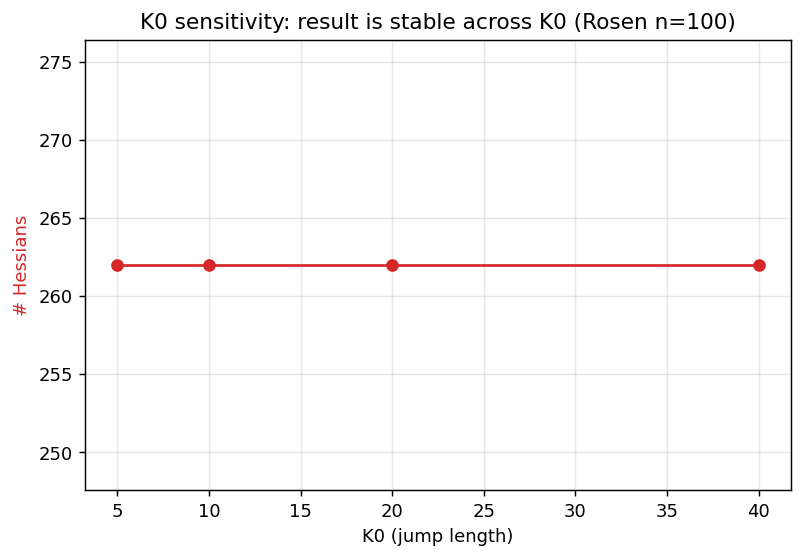
\includegraphics[width=0.8\linewidth]{figures/sensitivity_K0.png}
\caption{Robustness to the user-defined jump length $K_0$.}
\label{fig:k0}
\end{figure}

\begin{figure}[H]
\centering

\includegraphics[width=0.8\linewidth]{figures/sensitivity_tau.png}
\caption{Accuracy vs Hessian economy trade-off as a function of $\tau$.}
\label{fig:tau}
\end{figure}

\section{Conclusion and Future Work}
\label{sec:concl}

We proposed $\cn$, a stage-wise switching framework that keeps accelerated gradient and
Newton phases disjoint and switches on a geometric measure. The method is globally robust
and often succeeds where vanilla Newton, Newton--CG, and L-BFGS fail, especially in the
moderate-dimensional regime. It is insensitive to the jump length $K_0$ and offers a clean
$\tau$ trade-off.

Future work will (i)~move to the large-$n$ regime using Hessian-vector products so that
full Newton is unnecessary; (ii)~establish rigorous convergence of the checkpoint
subsequence $\{x_{jK}\}$ and the two-phase decay of the decrement; and (iii)~release an
open-source, reproducible package.

\begin{thebibliography}{9}

\bibitem{icn2026}
Inertial cubic-regularized Newton (ICN), \emph{NOLTA} 17, 2026.

\bibitem{optami2025}
Accelerated cubic Newton and accelerated tensor methods (OPTAMI/NATA), \emph{ICLR}, 2025.

\bibitem{aistats2025}
Momentum-accelerated stochastic cubic regularization, \emph{AISTATS}, 2025.

\bibitem{nesterov1983}
Y.~Nesterov, A method of solving a convex programming problem with convergence rate
$\mathcal{O}(1/k^2)$, \emph{Soviet Math.\ Dokl.}, 27:372--376, 1983.

\bibitem{nesterovpolyak2006}
Y.~Nesterov and B.~T.~Polyak, Cubic regularization of Newton's method and its global
performance, \emph{Math.\ Program.}, 108(1):177--205, 2006.

\bibitem{nocedal2006}
J.~Nocedal and S.~J.~Wright, \emph{Numerical Optimization}, 2nd ed., Springer, 2006.

\end{thebibliography}

\end{document}
